\lab{Naive Bayes}{Naive Bayes}
\label{Ch:NaiveBayes}


\objective{Implement Naive Bayes Classification Models}

%Outline
%
%Brief overview
%	With/Without independence assumptions
%	
%Types of Naive Bayes models
%	Multinomial
%	Gaussian
%	
%Simple Examples
%	Multinomial - Fair vs Loaded Dice
%		Dataset - generated by me
%	
%	Gaussian - Wheat Kernels
%		UCI Machine Learning
%		Sample test from training
%
%Application: spam Filtering
%	Dataset - Emails
%	Build wordcounts and labels
%	Sample test from training

\subsection*{Introduction}

Naive Bayes classification methods are a good introduction to machine learning techniques.
They are relatively straightforward to understand and implement, yet they are very effective for certain applications.
They are limited by their strong independence assumptions.

Recall that the classification problem tries to assign the correct label to a set of features
(called a \emph{feature vector}).
For example, suppose we wish to label two pieces of fruit with their correct names.
The first fruit is red and round, and the second fruit is long and yellow.
These attributes of the fruit are the features.
If we assign the names apple and banana respectively, then these are our labels.

It is common in classification problems to start with a set of labeled feature vectors called a training set.
We use the training set to train our algorithm to make predictions.
It is also common to have another smaller set of labeled feature vectors called a test set.
To verify the effectiveness of our algorithm, we predict the labels of the test set, and then compare the predicted labels to the true labels.

Now recall Bayes rule for random variables:
\[
P(Y|X) = \frac{P(X|Y)P(Y)}{\int P(X|Y)P(Y) dy}
\]
Where $P(Y)$ is our prior distribution and $P(X|Y)$ is our likelihood function.

Suppose that we have a set of features that we wish to label.
Let $x = (x_1, \ldots, x_n)$ be a feature vector and let $C = {c_1, \ldots, c_k}$ be our set of labels.
We may apply Bayes rule to this problem as follows:
\[
P(c_i|x) = P(c_i | x_1, \ldots, x_n)  = \frac{P(x_1, \ldots, x_n|c_i)P(c_i)}{P(x_1, \ldots, x_n)}
\]
If we make no further assumptions, this problem is intractable.
To effectively estimate even a case where each feature is a boolean value would require us to estimate around $k2^{n}$ parameters.
The problem gets exponentially worse if we were to consider non-boolean features.

However, if we make the assumption that features are conditionally independent from each other, the problem simplifies dramatically.
If we make this assumption and apply Bayes rule, we have
\[
P(c_i | x_1, \ldots, x_n) = \frac{P(x_1|c_i)P(x_2|c_i)\ldots P(x_n|c_i)P(c_i)}{P(x_1,\ldots,x_n)}
\]
In this case, we only need to estimate $kn$ parameters.
The naive Bayes classification algorithm chooses the label with the highest probability.
Since this is independent of the denominator in Bayes rule, we can simplify the problem further.
Given an unlabeled feature vector $x=(x_1,\ldots,x_n)$, we assign the label
\[
c = \underset{i \in \{1, \ldots, k\}}{\argmax}\, P(c_i)\prod_{j=1}^n P(x_j|c_i)
\]

To assign a label to a set of features, we calculate each $P(x_j|c_i)$ and choose a prior $P(c_i)$.
We then choose the argmax as above.
The calculation of conditional probabilities and choice of prior will depend on the type of problem that we are solving.

\subsection*{Gaussian Classifiers}

Gaussian classifiers are commonly used when dealing with continuous data.
We assume that each feature is normally distributed and conditionally independent.
We may then calculate $\mu_{j,i}$ and $\sigma^2_{j,i}$ corresponding to each feature of each class.
Then $P(x_j|c_i)$ can be calculated using the gaussian pdf
\[
P(x_j|c_i) = \frac{1}{\sqrt{2\pi\sigma_{j,i}^2}}\exp{-\frac{(x_j - \mu_{j,i})^2}{2\sigma^2_{j,i}}}
\]

For example, suppose we have a training set with labels indicating the sex of a person (1 for female, 2 for male), and  features consisting of hair length and height (features 1 and 2, respectively).
Further suppose that the mean height of the men in the training set is 1.75 meters with standard deviation 7 cm, and mean hair length is 5 centimeters with standard deviation 2.5 cm.
Similarly, suppose that the mean height of the women in the training set is 1.25 meters with standard deviation 6 cm, and the mean hair length is 15 centimeters with standard deviation 1.5 cm.
Under this setup, we have
\begin{align*}
\mu_{1,1} &= 15, \quad &&\sigma_{1,1} = 1.5\\
\mu_{2,1} &= 1.25, &&\sigma_{2,1} = .06\\
\mu_{1,2} &= 5, &&\sigma_{1,2} = 2.5\\
\mu_{2,2} &= 1.75, &&\sigma_{2,2} = .07.
\end{align*}
If we wish to classify a person that is 1.4 meters tall and a hair length of 17 centimeters, we calculate the probability of each label using the parameters given above and a uniform prior ($P(F) = P(M) = \frac{1}{2}$):
\begin{align*}
P(F\,|\,17,1.4) &= P(F)\left(\frac{1}{\sqrt{2\pi\sigma_{1,1}^2}}\exp{-\frac{(17-\mu_{1,1})^2}{2\sigma^2_{1,1}}}\right)
\left(\frac{1}{\sqrt{2\pi\sigma_{2,1}^2}}\exp{-\frac{(1.4-\mu_{2,1})^2}{2\sigma^2_{2,1}}}\right)\\
&= .016\\
P(M\,|\,17,1.4) &= P(M)\left(\frac{1}{\sqrt{2\pi\sigma_{1,2}^2}}\exp{-\frac{(17-\mu_{1,2})^2}{2\sigma^2_{1,2}}}\right)
\left(\frac{1}{\sqrt{2\pi\sigma_{2,2}^2}}\exp{-\frac{(1.4-\mu_{2,2})^2}{2\sigma^2_{2,2}}}\right)\\
&= 1.7\times 10^{-11}
\end{align*}
The Female label has a greater probability given the feature vector, and so we classify the person as Female.

A nice way to visualize how a classifier works is to plot the decision boundaries for two-dimensional subspaces of the
feature vector space.
For example, the decision boundaries for a Gaussian Naive Bayes classifier trained on a dataset consisting of the
sepal widths and lengths of three different types of flowers is shown in Figure \ref{fig:decision_boundary}.

\begin{figure}
	\centering
	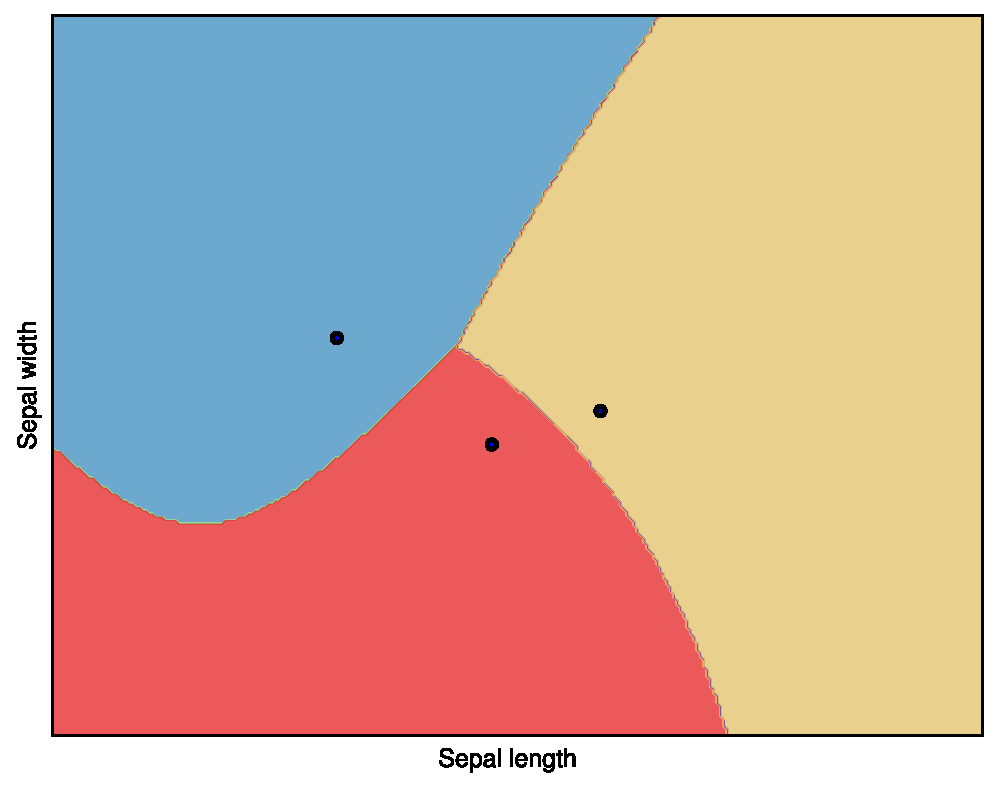
\includegraphics[width=.90\textwidth]{decision_boundary}
	\caption{Decision boundaries for a Gaussian Naive Bayes classifier on the iris flower dataset, together with the means
for each flower. Each point in the plane represents a 2-dimensional feature vector, and the color associated with each point indicates which class label was assigned to that feature vector.}
	\label{fig:decision_boundary}
\end{figure}

\subsection*{Working in Log Space}
In the example presented above, notice that the value of $P(M\,|\,17,1.4)$ is very small.
This is often the case in classification problems; certain classes may be very unlikely, and so calculating these probabilities may lead to numerical underflow.
This is especially pronounced in the naive Bayes model, which involves taking the product of several numbers between
0 and 1.
A useful technique to avoid underflow is to convert the computations in logarithmic space.
When we do so, the Naive Bayes label assignment is
\[
c = \underset{i \in \{1, \ldots, k\}}{\argmax}\, \log P(c_i) + \sum_{j=1}^n \log P(x_j|c_i).
\]
Since the logarithm is a monotone increasing function, the argmax is the same whether in log space or
in the original formulation.

\begin{problem}
Download the {\tt seeds\_dataset.txt} file.
This file contains 7 features describing 3 species of wheat.
\begin{enumerate}
\item Area
\item Perimeter
\item Compactness
\item Length
\item Width
\item Asymmetry Coefficient
\item Groove length
\end{enumerate}

The species of wheat are
\begin{enumerate}
\item Kama
\item Rosa
\item Canadian
\end{enumerate}

The measurements of the kernels are real valued, making this a good example to try our Gaussian classifier.

\begin{enumerate}
\item Randomly select a test set of 40 vectors from the data.  Make sure you separate this data from your training data.
\item Calculate the mean and variance for each feature of each label using the training set.
\item Using a uniform prior, predict the labels of your test set.
\item Compare your predictions to the labels of the test set. In particular, report the accuracy of the prediction,
which is the number of correctly predicted instances divided by the total number of instances.
\end{enumerate}

\end{problem}

We may also use SciPy's {\tt sklearn} library to implement a Gaussian classifier.
After importing the library, we can create a new classifier and train it with just a couple of lines of code.
To create a Gaussian classifier, use the following code.

\begin{lstlisting}
from sklearn.naive_bayes import GaussianNB
nb_classifier = GaussianNB()
\end{lstlisting}

Given a training set, we can also quickly train the classifier to a certain problem.
This requires the training set and labels as two arguments.

\begin{lstlisting}
nb_classifier.fit(training_set, labels)
\end{lstlisting}

Once the classifier has been trained, we can predict the labels for a test set.

\begin{lstlisting}
pred_labels = nb_classifier.predict(test_set)
\end{lstlisting}

The {\tt predict} method returns an array of labels for the test set.

\begin{problem}

Repeat the previous problem using {\tt sklearn}'s naive Bayes classifier.
Check that your implementation predicts the same labels as the {\tt sklearn}
implementation.

\end{problem}


\subsection*{Document Classification and spam Filters}

Naive Bayes classifiers are often used in document classification, a major example being spam detection.
When it comes to document classification, a common choice for the feature vector
is simply a count for the number of times each word in the specified vocabulary occurs in the document.
For example, suppose we are trying to classify a document, and the vocabulary of relevant words is the ordered set
\[
\text{(bank, tree, wealth, money, river, water)}.
\]
Suppose that the document is the sentence
\begin{quotation}
``The woman deposited her money in the bank, and then made her way down to the bank of the river, contemplating her wealth."
\end{quotation}
Then the feature vector for this document is
\[
(2, 0, 1, 1, 1, 0).
\]
Notice in particular that the $i$-th entry of the feature vector indicates the number of occurrences of the $i$-th
vocabulary word in the document.
Such a feature vector is often called a \emph{word-count vector}.
Notice that the count vector ignores words in the document that are not part of the vocabulary, and
it also disregards the order of words.
This simple representation of text documents is known as the \emph{bag-of-words model} or the \emph{vector space model}.
The hypothesis that drives spam filters is that spam messages will use words with different frequencies.
For example, a spam message will often have a sales pitch, so the word ``buy'' and ``cheap'' will appear often.
On the other hand, legitimate messages will probably use different language.
Thus, it is reasonable to use word-count vectors as our feature vectors when attempting to distinguish between spam and
legitimate email.

We now introduce formalisms to derive the Naive Bayes model for document classification.
Let $V = (v_1,v_2,\ldots,v_n)$ be an ordered list of words, called the vocabulary, and let
$x = (x_1,x_2,\ldots,x_n)$ be a word-count vector.
Let $\{c_1,c_2,\ldots,c_k\}$ be the set of classification labels.
In the case of continuous data and Gaussian Classifiers, each class label was associated with corresponding
mean and variance parameters, and these determined the likelihood of the feature vector given the class label.
In the case of document classification, each class label $c_i$ has a corresponding probability vector
$(p_{i,1}, p_{i,2}, \ldots, p_{i,n})$ whose entries are nonnegative and sum to 1.
This probability vector defines a categorical probability distribution over the vocabulary $V$, where $p_{i,j}$
represents the probability of seeing word $v_j$ given class label $c_i$.
With this notation in place, our Naive Bayes model takes the form
\[
c = \underset{i \in \{1, \ldots, k\}}{\argmax}\, P(c_i)\prod_{j=1}^n p_{i,j}^{x_j}.
\]

Given a training set of labeled documents, we can calculate the prior probabilities $P(c_i)$ and word probabilities
$p_{i,j}$ as follows.
Each prior probability $P(c_i)$ is simply the proportion of training documents that have the label $c_i$.
Next, let $count(c_i,v_j)$ denote the number of occurrences of word $v_j$ among all training documents that have label $c_i$. 
Then we have
\[
p_{i,j}  = \frac{count(c_i,v_j)+1}{\sum_{j=1}^n(count(c_i,v_j)+1)}.
\]
(Note that adding 1 to the number of occurrences of each word is known as \emph{add-one smoothing}, and is a
common technique to prevent over-fitting.)

Once we have calculated these parameters (the ``fitting" stage), we are ready to classify new documents
(the ``prediction" stage) using the argmax equation given above.
Remember to perform calculations in log-space to prevent numerical underflow.

\begin{problem}
Implement a Naive Bayes model for document classification.
We provide an interface below.

\begin{lstlisting}
class naiveBayes(object):
    """
    This class performs naive bayes classification for word-count document features.
    """
    def __init__(self,smoothed=False):
        """
        Initialize a naive Bayes classifier.
        """
        pass

    def fit(self,X,Y):
        """
        Fit the parameters according to the labeled training data (X,Y).

        Parameters
        ----------
        X : ndarray of shape (n_samples, n_features)
            Each row is the word-count vector for one of the documents
        Y : ndarray of shape (n_samples,)
            Gives the class label for each instance of training data. Assume class labels
            are in {0,1,...,k-1} where k is the number of classes.
        """
        # get prior class probabilities P(c_i)
        # (you may wish to store these as a length k vector as a class attribute)

        # get (smoothed) word-class probabilities
        # (you may wish to store these in a (k, n_features) matrix as a class attribute)

        pass

    def predict(self, X):
        """
        Predict the class labels of a set of test data.

        Parameters
        ----------
        X : ndarray of shape (n_samples, n_features)

        Returns
        -------
        Y : ndarray of shape (n_samples,)
            Gives the classification of each row in X
        """
        pass
\end{lstlisting}
\end{problem}

\begin{problem}
In this problem, you will train a Naive Bayes classifier using a corpus of emails extracted from the Enron dataset.

Load in the data from {\tt SpamFeatures.txt}. This is a text file containing a whitespace-delimited
numerical array with several thousand columns and several thousand rows, each row representing an email
as a count vector.
Also load in the data from {\tt SpamLabels.txt}, which is a text file containing a 1 (for legitimate email) or 0
(for spam email) on each line, in correspondence with the rows of the count vector array.
Using your document classification implementation, do the following:
\begin{enumerate}
\item Randomly create a test set from the data (500 documents), leaving the remaining documents as the training set.
\item Create a naive Bayes classifier and fit it using the training set.
\item Predict the labels of the test set and compare to the true labels (by reporting the classification accuracy).
\end{enumerate}

Next, perform the same task using {\tt sklearn}'s implementation and the same train and testing sets:
\begin{lstlisting}
>>> # assume train_vectors, train_labels, and test_vectors are defined
>>> from sklearn.naive_bayes import MultinomialNB
>>> mnb = MultinomialNB()
>>> mnb.fit(train_vectors, train_labels)
>>> predicted = mnb.predict(test_vectors)
\end{lstlisting}
Again report the accuracy of the predicted labels. The result should be on par with those produced by your
own implementation.

If you wish, you may use your Naive Bayes classifier on your own email.
To do so, you need to load in the words in the vocabulary, contained in the file {\tt SpamVocab.txt}, as follows:
\begin{lstlisting}
>>> with open("SpamVocab.txt", 'r') as f:
>>>     vocab = [s.strip() for s in f]
\end{lstlisting}
Next, load the email you wish to classify into memory, stored as a string object (either copy and paste the email
directly into the interpreter, or load it from a file). Once you have this string, convert it to a count vector using
the following code:
\begin{lstlisting}
from collections import Counter
def getCountVector(document, vocab):
    """
    Return the count vector for the given document using the given vocabulary.

    Parameters
    ----------
    document : string, words separated by whitespace
    vocab : list of strings of length n

    Returns
    -------
    counts : ndarray of shape (1,n)
    """
    tf = Counter(document.lower().split()) # get frequencies of each word
    counts = np.array([[tf[t] if t in tf else 0 for t in vocab]])
    return counts
\end{lstlisting}
Feed this output into the \li{predict} method of your classifier, and see how well it performs.
\end{problem}


\begin{comment}
I didn't find this section to be necessary. I wanted to jump right to full document classification.

A good analogy to help us understand is the problem of classifying dice as fair or loaded.
Suppose that we had 100 rolls from 1000 different dice.
Some dice are fair, but other dice favor rolls of 3 or 4.
Our task is to identify unlabeled dice as either fair or weighted.
We could generate such an experiment in python as follows.

\begin{lstlisting}

#Generate 100 rolls from 1000 dice, some fair and some weighted
#All weighted dice favor 3 and 4

import numpy as np
import random

prob_fair = 0.7
num_dice = 1000
num_rolls = 100

fair_die = np.array([1, 2, 3, 4, 5, 6])
weighted_die = np.array([1,2,3,3,3,3,4,4,4,4,5,6])

rolls = np.zeros((num_dice, num_rolls))
label = np.zeros((num_dice,1))

for i in xrange(num_dice):
    if np.random.random() < prob_fair:
        for j in xrange(num_rolls):
            rolls[i,j] = random.choice(fair_die)
        label[i] = 0
    else:
        for j in xrange(num_rolls):
            rolls[i,j] = random.choice(weighted_die)
        label[i] = 1

\end{lstlisting}

In this case, {\tt rolls} is a matrix whose rows are rolls from either a fair or a loaded die.
Our labels are stored in {\tt label}.
We can build a multinomial naive Bayes classifier using {\tt sklearn}.

\begin{lstlisting}
from sklearn.naive_bayes import MultinomailNB
mnb_classifier = MultinomialNB
mnb_classifier.fit(rolls,label)
\end{lstlisting}

The multinomial classifier trains on the roll data on each line.
We can now predict whether a new set of die rolls is either fair or loaded.

\begin{lstlisting}
roll = np.random.randint(1,7,size=100)
mnb.predict(roll)
\end{lstlisting}

\begin{problem}
The die roll problem is simplification of a spam filter.
The different kinds of die produce different kinds of rolls.
Thus, the probability of getting one kind of histogram of rolls is different depending on the label of the die.
Write an explanation of how you could extend these ideas to a spam filter, and how you would use {sklearn} to implement it.
\end{problem}
\end{comment}

